\subsection{Descripci\'on del problema}

Tenemos un juego de un solo jugador, el cual consta de un tablero como el de ajedrez, con la diferencia de que el tablero tiene un tamaño de $n x n$ casillas, y las piezas con las que se juegan son solo caballos. El juego comienza con una cantidad k de caballos blancos repartidos, sin ninguna particularidad, por todo el tablero. Y el objetivo del juego es encontrar (en caso de que el juego tenga solucion), un casillero donde poder ubicar todos los caballos del tablero, habiendo hecho la menor cantidad de movimientos posibles. 
Algunas aclaraciones:
\begin{itemize}
\item El movimiento de los caballos es igual al movimiento de los mismos en el juego de ajedrez, en forma de "L", la imagen 1.
\item En todo momento puede haber mas de un caballo en la misma casilla del tablero. El juego podria empezar con mas de un caballo en alguna casilla.
\item Un movimiento se cuenta como el movimiento de un caballo de una casilla a otra.
\end{itemize}

\begin{figure}[H]
\begin{center}
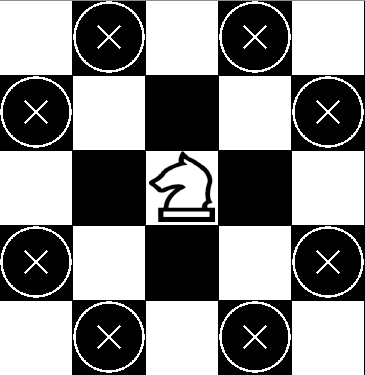
\includegraphics[scale=.45]{./imagenes/ej2_movimientoCaballo.png}
\caption{Img2: Movimientos posibles de un caballo en el tablero.}
\end{center}
\end{figure}

En la siguiente imagen mostramos el comienzo y la serie de movimientos de los caballos hasta llegar todos a una misma casilla. Para simplificar el ejemplo en cada imagen todos los caballos hacen un movimiento.

\begin{figure}[H]
\begin{center}
\includegraphics[scale=.45]{./imagenes/ej2_ejemploDeJuego.png}
\caption{Img2: Serie de movimientos optimos.}
\end{center}
\end{figure}


\subsection{Resoluci\'on}



\subsection{Demostraci\'on de la resoluci\'on}


\subsection{Complejidad del algoritmo}


\subsection{C\'odigo fuente}


\subsection{Casos de prueba}

Para este ejercicio pensamos varias instancias de prueba como las siguientes:

\begin{itemize}
\item Caso de un tablero de 2 x 2 con dos caballos ubicados en distintos casilleros. Este caso no tiene solucion, ya que el tablero no tiene un tamaño suficiente como para que alguno de los caballos realice un movimiento.
\item Caso de un tablero de (ver despues el tamaño) con 4 caballos ubicados en cada una de las puntas del tablero. Aquí la solución tiene que dar el casillero que se encuentra justo en el medio del tablero.
\item Caso de un tablero (en el que no importa el tamaño) con un solo caballo. En este caso como solo hay un caballo, no seria necesario mover el caballo ya que es el único del tablero.
\item Caso 3 con 2 caballos. Este caso es igual al caso anterior, solo que hay dos caballos en la misma casilla. Al igaul que en el caso anterior, la optimicidad se obtiene no realizando ningun movimiento, osea, con una cantidad de movimientos igual a cero.
\item
\end{itemize}

\subsection{Performance}



\begin{figure}[H]
\begin{center}
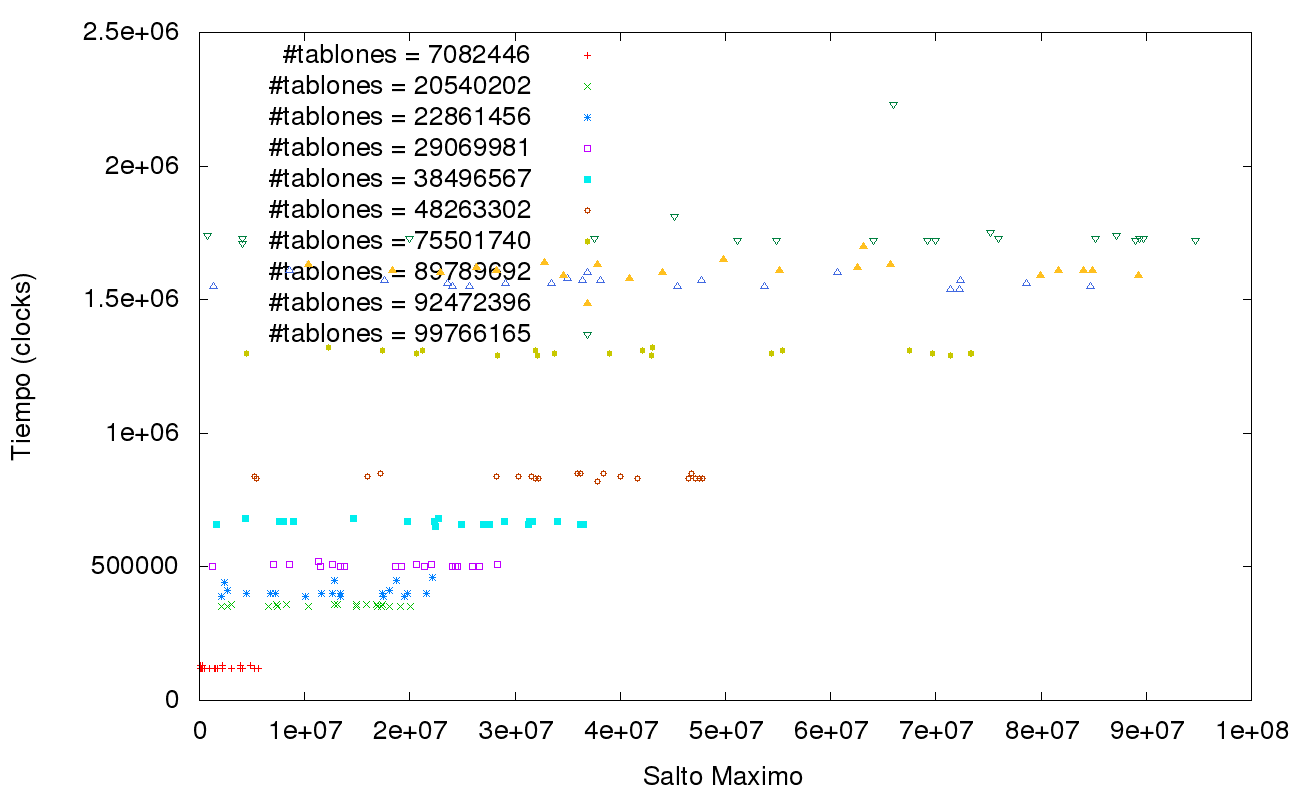
\includegraphics[scale=.45]{./imagenes/ej1_testSaltoMaximo.png}
\caption{Gr\'afico de tiempo en funci\'on del salto m\'aximo.}
\end{center}
\end{figure}

